\documentclass{standalone}
\usepackage{tikz}
\usepackage{ctex,siunitx}
\usepackage{tkz-euclide}
\usepackage{amsmath}
\usetikzlibrary{patterns, calc}
\usetikzlibrary {decorations.pathmorphing, decorations.pathreplacing, decorations.shapes,}
\begin{document}
\small
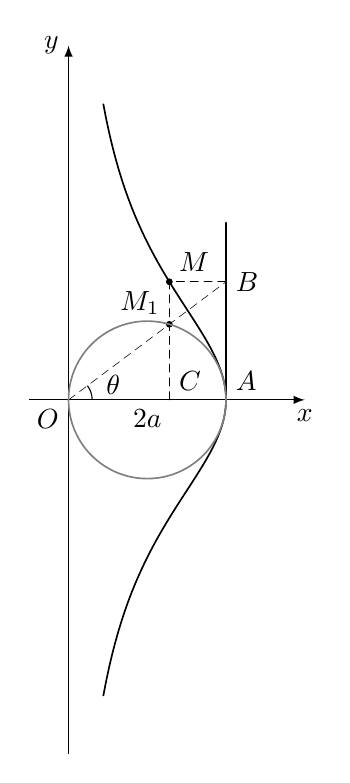
\begin{tikzpicture}[>=latex,scale=1]
  \draw[thin,->](-0.5,0)--(3,0)node[below]{$x$};
  \draw[thin,->](0,-4.5)--(0,4.5)node[left]{$y$};
  \tkzDefPoints{0/0/O,2/0/A,2/1.5/B,1/0/P}
  \tkzInterLC(O,B)(P,A)\tkzGetPoints{M1}{M2}
  \tkzDefPointBy[projection=onto O--A](M1)\tkzGetPoint{C}
  \tkzDefPointBy[translation=from A to B](C)\tkzGetPoint{M}
  \draw[semithick,domain=-62:62,samples=100] plot ({2*cos(\x)*cos(\x)},{2*tan(\x)});
  \tkzDrawLine[semithick,add=0 and 0.5](A,B)
  \tkzDrawSegments[densely dashed](B,M C,M O,B)
  \tkzDrawPoints[fill=black](M,M1)
  \tkzDrawCircle[semithick](P,A)
  \tkzMarkAngle[size=0.3](A,O,B)
  \tkzLabelAngle[pos=0.6](A,O,B){$\theta$}
  \tkzLabelPoints[right](B)
  \tkzLabelPoints[above right](A,M,C)
  \tkzLabelPoints[below left](O)
  \tkzLabelPoint[above left](M1){$M_1$}
  \node at (1,0)[below]{$2a$};
\end{tikzpicture}
\end{document}